%%
%% Paper 1 — Threshold Selection as a Critical Design Choice in Financial Fraud Detection
%% Target venue: Expert Systems with Applications (Elsevier)
%%
%% REVISED VERSION (writing-only pass; experiments, numbers, tables, citations untouched)
%%

\documentclass[a4paper,fleqn]{cas-sc}

\usepackage[authoryear,longnamesfirst]{natbib}
\usepackage{booktabs}
\usepackage{multirow}
\usepackage{xcolor}
\usepackage{colortbl}
\usepackage{amsmath}
\usepackage{graphicx}
\usepackage{enumitem}
\usepackage{capt-of}  % \captionof for non-floating tables and figures

%% Consistent model colours (match thesis figures)
\definecolor{clrLGBM}{HTML}{1f77b4}
\definecolor{clrCB}{HTML}{d62728}
\definecolor{clrRF}{HTML}{2ca02c}
\definecolor{clrFT}{HTML}{ff7f0e}
\definecolor{clrLR}{HTML}{9467bd}

\begin{document}
\let\WriteBookmarks\relax
\def\floatpagepagefraction{1}
\def\textpagefraction{.001}

%% ─── Front matter ──────────────────────────────────────────────────────────

\shorttitle{Threshold Selection in Financial Fraud Detection}

\shortauthors{Caixeiro et al.}

\title[mode=title]{Threshold Selection as a Critical Design Choice in Financial Fraud Detection:
  A Systematic Comparison of Classical Machine Learning Models and Tabular Transformers}

\author[1]{Olavo Caixeiro}[
  orcid=0009-0004-1532-4830,
]
\cormark[1]
\ead{200100274@esg.ipsantarem.pt}
\credit{Conceptualization, Methodology, Software, Formal analysis, Writing -- original draft}

\author[1]{Maryam Abbasi}[
  orcid=0000-0002-9011-0734,
]
\ead{maryam.abbasi@esg.ipsantarem.pt}
\credit{Conceptualization, Supervision, Writing -- review \& editing}

\author[1]{Pedro Martins}[
  orcid=0000-0001-9600-082X,
]
\ead{pedro.martins@esg.ipsantarem.pt}
\credit{Supervision, Writing -- review \& editing}

\affiliation[1]{
  organization={Departamento de Inform\'atica e M\'etodos Quantitativos,
    Escola Superior de Gest\~ao e Tecnologia,
    Instituto Polit\'ecnico de Santar\'em},
  city={Santar\'em},
  country={Portugal}
}

\cortext[1]{Corresponding author}

%% ─── Abstract ──────────────────────────────────────────────────────────────

\begin{abstract}
The evaluation of fraud detection models under extreme class imbalance is shaped less
by the choice of classifier than by the behaviour of model scores in the regime where
positives are scarce. Under this regime, output probabilities are systematically
compressed towards zero, and the decision threshold that converts those probabilities
into operational decisions becomes the dominant lever controlling detection performance.
Yet across the literature this threshold is typically left at the scikit-learn default
of~$\tau=0.5$ or selected on the test set, both of which inflate reported metrics and
preclude fair comparison across model families.
This paper develops a leakage-free experimental framework in which the decision threshold
is treated as a first-class experimental variable, calibrated exclusively on inner
validation folds, and never reused from the held-out test set.
Six model families --- Logistic Regression, Random Forest, LightGBM, CatBoost,
One-Class SVM, and FT-Transformer --- are compared under seven class imbalance handling
strategies and four threshold selection strategies on two structurally distinct
benchmarks: the ULB Credit Card Fraud dataset ($N\!=\!284{,}807$, $0.17\%$ fraud) and
the Bank Account Fraud (BAF) Base dataset ($N\!=\!1{,}000{,}000$, ${\approx}1.1\%$ fraud).
The two benchmarks exhibit qualitatively different score geometries.
On ULB, predicted scores are well-separated and the fixed default is close to optimal,
with CatBoost leading at PR-AUC~$=\!0.885$.
On BAF, scores cluster well below~$0.5$ and the fixed default is operationally unsuitable:
$F_2$ falls below~$0.04$ for every supervised model, whereas a max-$F_2$ threshold
calibrated on validation folds recovers $F_2$ values in the $0.29$--$0.32$ range, an
improvement of up to nine-fold without retraining.
No single imbalance handling strategy uniformly dominates, and Class~Weights emerges as
the safest default; SMOTE+Tomek Links coincides exactly with SMOTE under this prevalence
regime, since no borderline majority examples remain for Tomek to remove.
At the BAF scale, the FT-Transformer matches CatBoost at PR-AUC~$=\!0.180$ but at
substantially higher computational cost, indicating that tabular transformers are
competitive rather than superior to well-tuned gradient boosting.
A decision framework maps seven deployment scenarios to recommended
model--strategy--threshold configurations.
\end{abstract}

%% ─── Highlights ────────────────────────────────────────────────────────────

\begin{highlights}
\item Score compression under extreme imbalance renders the fixed default $\tau{=}0.5$ operationally unsuitable on large-scale bank account fraud data
\item Validation-calibrated max-$F_2$ thresholds achieve up to $9{\times}$ $F_2$ improvement over the fixed default without retraining
\item SMOTE and SMOTE+Tomek Links coincide under extreme imbalance, as no borderline majority examples remain for Tomek to remove
\item Class~Weights is the safest default imbalance strategy across model families
\item A decision framework links seven deployment scenarios to recommended model--strategy--threshold configurations
\end{highlights}

%% ─── Keywords ──────────────────────────────────────────────────────────────

\begin{keywords}
  fraud detection \sep threshold selection \sep class imbalance \sep gradient boosting
  \sep tabular transformers \sep precision-recall \sep FT-Transformer
\end{keywords}

\maketitle

%% ════════════════════════════════════════════════════════════════════════════
\section{Introduction}
\label{sec:intro}
%% ════════════════════════════════════════════════════════════════════════════

Electronic payment fraud causes annual global losses in the hundreds of billions of
dollars, and the continued proliferation of digital payment channels has expanded the
attack surface that adversaries can exploit \citep{rymantubb2018survey}.
Automated detection systems trained on historical transaction records have therefore
become a structural component of how financial institutions defend their portfolios.
The underlying learning problem, however, sits at an unfavourable intersection of three
properties: fraud prevalence is typically between $0.1\%$ and $2\%$
\citep{hegarcia2009learning}; the data-generating process is non-stationary, since
fraud patterns adapt to the systems deployed against them; and misclassification costs
are strongly asymmetric, with missed fraud translating into direct financial losses and
false alerts into investigator workload and customer friction.

Within this setting, a recurrent methodological weakness in the published literature
has limited the practical reliability of reported results. The most consequential is
\emph{data leakage}: resampling applied prior to the train/test split, or applied across
folds rather than within them, inflates reported metrics by margins large enough to
reverse model rankings \citep{hayat2025leakage}. A second issue concerns the choice of
summary metric: ROC-AUC remains widely reported but is insensitive to the class prior,
and under severe imbalance can take values above~$0.95$ while the model still fails to
recover most fraud cases \citep{saito2015precision}. A third issue, less discussed in
the literature, concerns the decision threshold itself. The threshold $\tau$ that
converts a probability score into a binary fraud decision is rarely treated as an
experimental variable; instead, it is fixed at the scikit-learn default of~$0.5$ or,
worse, selected by inspecting the test set.

A clearer way to frame the problem is to think in terms of score geometry. Under extreme
imbalance, supervised classifiers tend to produce probability distributions in which
even genuine fraud receives scores well below~$0.5$, so the operating point implied by
the default threshold sits in a region of the probability simplex where almost no
fraud is detected. The behaviour of a fraud detector is therefore determined as much
by the interaction between the score distribution and the threshold rule as by the
underlying model. Despite its operational centrality, this interaction has not been
systematically characterised across model families and datasets under a strict
leakage-free protocol.

This paper addresses that gap. Specifically, it makes four contributions. The first is
a reproducible, leakage-free evaluation protocol applied to six model families on two
structurally distinct fraud datasets (ULB and BAF), eliminating leakage at every stage
of resampling, threshold selection, and hyperparameter tuning. The second is the
treatment of threshold selection as a primary experimental variable: four threshold
selection strategies (fixed~$\tau=0.5$, max-$F_1$, max-$F_2$, and Precision~$\geq 0.5$)
are calibrated exclusively on inner validation folds, and their impact on both metrics
and rankings is quantified. The third is a full factorial analysis of seven class
imbalance handling strategies in a $7{\times}5{\times}2$ design, identifying which
interventions help, harm, or leave performance unchanged. The fourth is a decision
framework that maps seven representative deployment scenarios to recommended
model--strategy--threshold configurations.

The remainder of this paper is organised as follows.
Section~\ref{sec:relwork} surveys the relevant literature on fraud detection evaluation,
class imbalance, and threshold selection.
Section~\ref{sec:framework} describes the experimental framework.
Section~\ref{sec:results} presents the experimental results.
Section~\ref{sec:discussion} interprets the main findings and develops the decision
framework.
Section~\ref{sec:conclusion} concludes and outlines directions for future work.

%% ════════════════════════════════════════════════════════════════════════════
\section{Related Work}
\label{sec:relwork}
%% ════════════════════════════════════════════════════════════════════════════

\subsection{Fraud Detection Benchmarks and Evaluation under Class Imbalance}

The ULB Credit Card Fraud dataset \citep{dalpozzolo2015calibrating, dalpozzolo2017realistic}
has been the de facto benchmark in the field for more than a decade, although its
PCA-anonymised features rule out any domain-level interpretation.
The Bank Account Fraud (BAF) suite \citep{jesus2022turning}, released at NeurIPS~2022,
addresses this limitation by providing one million synthetic but feature-rich bank
account applications with semantic variable names, a ${\approx}1.1\%$ fraud prevalence,
and five distribution-shifted variants designed to stress-test robustness under
covariate shift, label shift, and subpopulation bias.
The two benchmarks are therefore complementary rather than redundant: ULB is small
($N\!=\!284\text{K}$) and privacy-constrained, while BAF is large-scale, semantically
rich, and explicitly designed for shift analyses.

The choice of evaluation metric is no less consequential than the choice of dataset.
\citet{saito2015precision} show that ROC-AUC is insensitive to the class prior and
therefore misleading under extreme imbalance, with values above~$0.95$ remaining
compatible with most fraud cases going undetected. The area under the precision-recall
curve (PR-AUC) is a more informative summary, as it directly traces the trade-off
between detection rate (recall) and false-alert burden (precision) across all
operating points \citep{saito2015precision, dalpozzolo2017realistic}. At deployment
time, the $F_\beta$-score \citep{rymantubb2018survey} is the more natural operational
metric, with $\beta\!=\!2$ widely adopted for fraud applications because the cost of
missing a fraud transaction typically exceeds the cost of investigating a false alert.

\subsection{Class Imbalance Handling Strategies}

The standard remedies for class imbalance in supervised learning fall into three
families: undersampling of the majority class, oversampling of the minority class, and
cost-sensitive learning that modifies the loss function. SMOTE \citep{chawla2002smote}
is the canonical oversampling method, generating synthetic minority examples by
interpolating between existing positives in feature space, and was later combined with
data-cleaning post-processors such as Tomek Links (SMOTE+Tomek) or Edited Nearest
Neighbours (SMOTEENN) by \citet{batista2004balancing}. The broader comparative
evidence \citep{hegarcia2009learning, fernandez2018smote} indicates that no single
strategy dominates across datasets and model families, which motivates factorial rather
than single-strategy evaluations.

A more subtle limitation of much of this literature is that the imbalance strategy and
the decision threshold are typically evaluated in isolation: the strategy is varied
while the threshold is held at~$0.5$ or chosen informally. This conflation prevents
attribution of performance differences to their true source, since the threshold that
is operationally optimal for the resulting score distribution may differ substantially
from~$0.5$, independently of whether oversampling was applied.

\subsection{Threshold Selection and Evaluation Integrity}

The decision threshold is the value above which a probability output is labelled fraud.
The scikit-learn default of~$0.5$ is calibrated for balanced binary classification and
carries an implicit assumption about the score distribution that is rarely satisfied
under extreme imbalance. Empirically, on large-scale bank account data the optimal
operating threshold lies in the~$0.05$--$0.10$ range, more than half an order of
magnitude below the default; applying~$\tau=0.5$ in that regime yields very few
positive predictions and a near-collapse of recall.

\citet{luzio2024decoupling} formally decouple threshold selection from model fitting
in the fraud detection context, showing that the separation removes an important source
of evaluation bias.
\citet{hayat2025leakage} catalogue leakage patterns in the published literature and
identify threshold selection on the test set as one of the most frequent sources of
inflated performance claims.
\citet{dalpozzolo2017realistic} compare threshold strategies on ULB and observe that
model rankings can change with the choice of threshold, yet this finding has not been
broadly absorbed into standard practice.

A parallel line of work has examined the relative standing of tabular deep learning
against gradient-boosted decision trees (GBDTs). \citet{shwartzziv2022tabular} report
that GBDTs consistently match or outperform tabular transformers on small-to-medium
tabular datasets. That comparison, however, was conducted without an explicit threshold
sensitivity component, leaving open whether the reported differences are stable across
operating points.

Against this background, the present paper provides what, to the best of our knowledge,
is the first joint leakage-free comparison of classical ML models and a tabular
transformer on both a small and a large-scale fraud benchmark in which threshold
selection is treated as a primary experimental variable rather than a post-hoc tuning step.

%% ════════════════════════════════════════════════════════════════════════════
\section{Experimental Framework}
\label{sec:framework}
%% ════════════════════════════════════════════════════════════════════════════

\subsection{Datasets}
\label{subsec:datasets}

Two structurally distinct fraud benchmarks are used, summarised in
Table~\ref{tab:data_chars}.

\par\medskip\noindent\begin{minipage}{\linewidth}\centering
\captionof{table}{Dataset characteristics.}
\label{tab:data_chars}
\begin{tabular}{l c c c c l}
\toprule
Dataset & $N$ & Fraud (\%) & Features & Type & Reference \\
\midrule
ULB 2013 & 284,807 & 0.17 & 30 & PCA + Amount & \citet{dalpozzolo2017realistic} \\
BAF Base & 1,000,000 & 1.09 & 30 & Semantic & \citet{jesus2022turning} \\
\bottomrule
\end{tabular}
\end{minipage}\par\medskip

The ULB Credit Card Fraud dataset covers European credit card transactions over two
days in September 2013, with 492 fraud cases out of 284{,}807 transactions ($0.172\%$).
Features V1--V28 are PCA components used for privacy preservation, accompanied by
\texttt{Time} and \texttt{Amount}. Because the predictors are anonymised, no
domain-level interpretation is possible on this dataset.
The Bank Account Fraud (BAF) Base dataset, generated using the simulation framework of
\citet{jesus2022turning} (NeurIPS 2022 Datasets Track), contains one million synthetic
bank account applications described by 30 semantic features (25 numerical and 5
categorical: \texttt{payment\_type}, \texttt{employment\_status}, \texttt{housing\_status},
\texttt{source}, \texttt{device\_os}), with a binary label \texttt{fraud\_bool} at a
prevalence of approximately $1.09\%$. Unlike ULB, the BAF features carry domain
meaning, which enables interpretability analyses.

\subsection{Models}
\label{subsec:models}

Six model families spanning the methodological range of contemporary tabular fraud
detection are evaluated. Logistic Regression with elastic-net regularisation
\citep{tibshirani1996regression} provides a linear lower-bound reference. Random Forest
\citep{breiman2001random} represents the bagged ensemble family, valued in particular
for its cross-domain robustness through feature subsampling. The gradient-boosted
family is represented by LightGBM \citep{ke2017lightgbm}, which combines leaf-wise tree
growth with histogram-based gradient computation, and by CatBoost
\citep{prokhorenkova2018catboost}, which adds ordered boosting and native categorical
handling and tends to deliver strong out-of-the-box performance on mixed-type tabular
data. One-Class SVM \citep{scholkopf2001estimating} is included as an anomaly-detection
baseline trained only on legitimate transactions, primarily to quantify the value of
supervised fraud labels relative to a purely unsupervised regime. Finally, the
FT-Transformer \citep{gorishniy2021revisiting} represents the most competitive tabular
deep learning architecture currently reported in the literature.

\subsection{Class Imbalance Handling Strategies}
\label{subsec:strategies}

Seven class imbalance handling strategies are evaluated for all supervised models (LR,
RF, LGBM, CB, FT-Transformer). The \emph{None} condition corresponds to no resampling
and serves as the baseline. Random Under-Sampling (RUS) and Random Over-Sampling (ROS)
respectively remove majority examples and duplicate minority examples at random.
SMOTE \citep{chawla2002smote} generates synthetic minority examples by interpolation in
feature space, and is also evaluated in its two post-processed forms
\citep{batista2004balancing}: SMOTE+Tomek, which removes Tomek-linked pairs after
oversampling, and SMOTEENN, which applies Edited Nearest Neighbour cleaning instead.
Finally, Class~Weights modifies the model's loss function by penalising minority-class
errors inversely to the class frequency.

One-Class SVM is excluded from the strategy comparison because it does not consume
fraud labels. All resampling strategies are applied exclusively within the training
partition of each cross-validation fold (see Section~\ref{subsec:protocol}) to prevent
resampling leakage. The full design yields $7 \times 5 = 35$ configurations per dataset
for the supervised models.

\subsection{Decision Threshold Strategies}
\label{subsec:threshold}

Rather than treating the decision threshold as an operational afterthought, this paper
treats it as a primary experimental variable. Four threshold strategies are evaluated
for each trained model. The first is the na\"{\i}ve fixed default $\tau=0.5$, which is
appropriate only when output scores are well-calibrated around $0.5$. The next two are
the validation-optimal $F_\beta$ thresholds, defined as
$\tau^{*} = \arg\max_{\tau} F_{\beta}(\tau)$ on the inner validation folds, evaluated
for $\beta=1$ (max-$F_1$, balanced precision--recall trade-off) and for $\beta=2$
(max-$F_2$, the primary criterion, which weights recall twice as heavily as precision).
The fourth strategy, Precision~$\geq 0.5$, selects the lowest $\tau$ such that
$\text{Precision}(\tau) \geq 0.5$ on the validation folds, simulating a hard workload
constraint of at most one false alert per genuine fraud.

All four strategies select $\tau$ exclusively on inner validation folds, and the
median $\tau$ across folds is applied to the held-out test set. Critically, the
threshold study reuses the trained models and probability scores from the baseline
(strategy\,=\,None); no retraining is performed, so the entire threshold sensitivity
analysis is obtained at no additional computational cost.

\subsection{Leakage-Free Evaluation Protocol}
\label{subsec:protocol}

A strict leakage-free protocol is enforced at three stages: resampling, preprocessing,
and threshold selection.

\textbf{Outer split.}
Each dataset is partitioned into an 80\% training partition (DEV) and a 20\% held-out
test set, stratified by class label. The test set is never examined during any
selection, fitting, or calibration step.

\textbf{Inner cross-validation.}
All model selection and threshold calibration occur within the DEV partition via
stratified 5-fold cross-validation. Within each fold, the preprocessor (imputation,
standardisation, one-hot encoding) is fitted on the fold's training subset only and
applied to the validation subset; resampling is applied only on the fold's training
subset; the model is trained on the resampled training subset; and the threshold
$\tau$ is selected on the fold's validation subset using the chosen strategy. The
median $\tau$ across the five folds is the threshold applied to the test set.

\textbf{Final evaluation.}
The model is retrained on the full DEV partition with the best hyperparameters, and
the median threshold from inner cross-validation is applied to the test set without
modification. Bootstrap 95\% confidence intervals ($B\!=\!1\,000$ iterations) are
computed on the test set for PR-AUC and ROC-AUC.

\subsection{Hyperparameter Optimisation}
\label{subsec:hpo}

All supervised models are tuned with Optuna \citep{akiba2019optuna} using the
Tree-structured Parzen Estimator (TPE) sampler and MedianPruner (50~trials, PR-AUC
objective). Classical models are tuned under stratified 5-fold cross-validation; the
FT-Transformer is tuned under a single 80/20 holdout within DEV. The best
hyperparameters identified under the baseline condition (strategy\,=\,None) are reused
for all resampling strategy experiments, so that the effect of the balancing technique
is isolated from changes in model capacity. The search spaces and the optimal
configurations per dataset are reported in the supplementary material.

\subsection{Evaluation Metrics}
\label{subsec:metrics}

PR-AUC, the area under the Precision--Recall curve, is the primary summary metric.
The $F_\beta$-score is the primary operational metric, with $\beta\!=\!2$ for the
threshold sensitivity study (recall-weighted) and $\beta\!=\!1$ for secondary analysis.
Recall (true positive rate) captures the fraction of fraud cases detected, and Alert
Rate, the fraction of transactions flagged as fraud, quantifies the operational workload
imposed on investigators. Bootstrap 95\% confidence intervals provide statistical
precision estimates for PR-AUC and ROC-AUC on the held-out test set.

%% ════════════════════════════════════════════════════════════════════════════
\section{Results}
\label{sec:results}
%% ════════════════════════════════════════════════════════════════════════════

\subsection{Baseline Model Comparison}
\label{subsec:baseline}

Tables~\ref{tab:baseline_ulb} and~\ref{tab:baseline_baf} report performance under the
baseline condition (strategy\,=\,None, threshold\,=\,max-$F_2$) on both datasets.
Figure~\ref{fig:prauc_baseline} draws the corresponding Precision--Recall curves and
overlays, for each supervised model, the four threshold-rule markers introduced in
Section~\ref{sec:framework}. The figure therefore offers a visual preview of the
threshold-sensitivity analysis that is formalised in
Section~\ref{subsec:threshold_results}.

\par\medskip\noindent\begin{minipage}{\linewidth}\centering
\captionof{table}{Baseline performance on ULB 2013 (strategy\,=\,None, threshold\,=\,max-$F_2$).}
\label{tab:baseline_ulb}
\begin{tabular}{l c c c c c c}
\toprule
Model & PR-AUC & ROC-AUC & $F_1$ & $F_2$ & Recall & Alert Rate \\
\midrule
LR         & 0.742 & 0.965 & 0.749 & 0.799 & 0.837 & 0.21\% \\
RF         & 0.867 & 0.959 & 0.831 & 0.858 & 0.878 & 0.19\% \\
LGBM       & 0.874 & 0.975 & 0.824 & 0.843 & 0.857 & 0.19\% \\
CatBoost   & 0.885 & 0.978 & 0.833 & 0.853 & 0.867 & 0.19\% \\
FT-Trans.  & 0.856 & 0.975 & 0.755 & 0.807 & 0.847 & 0.17\% \\
OCSVM      & 0.335 & 0.953 & 0.415 & 0.527 & 0.643 & 0.36\% \\
\bottomrule
\end{tabular}
\end{minipage}\par\medskip

\par\medskip\noindent\begin{minipage}{\linewidth}\centering
\captionof{table}{Baseline performance on BAF Base (strategy\,=\,None, threshold\,=\,max-$F_2$).}
\label{tab:baseline_baf}
\begin{tabular}{l c c c c c c}
\toprule
Model & PR-AUC & ROC-AUC & $F_1$ & $F_2$ & Recall & Alert Rate \\
\midrule
LR         & 0.143 & 0.875 & 0.187 & 0.287 & 0.445 & 4.14\% \\
RF         & 0.159 & 0.878 & 0.205 & 0.294 & 0.415 & 3.36\% \\
LGBM       & 0.177 & 0.899 & 0.222 & 0.316 & 0.439 & 3.25\% \\
CatBoost   & 0.180 & 0.898 & 0.211 & 0.314 & 0.468 & 3.80\% \\
FT-Trans.  & 0.180 & 0.897 & 0.225 & 0.316 & 0.434 & 3.16\% \\
OCSVM      & 0.019 & 0.628 & 0.045 & 0.081 & 0.171 & 7.32\% \\
\bottomrule
\end{tabular}
\end{minipage}\par\medskip

\par\medskip\noindent\begin{minipage}{\linewidth}\centering
  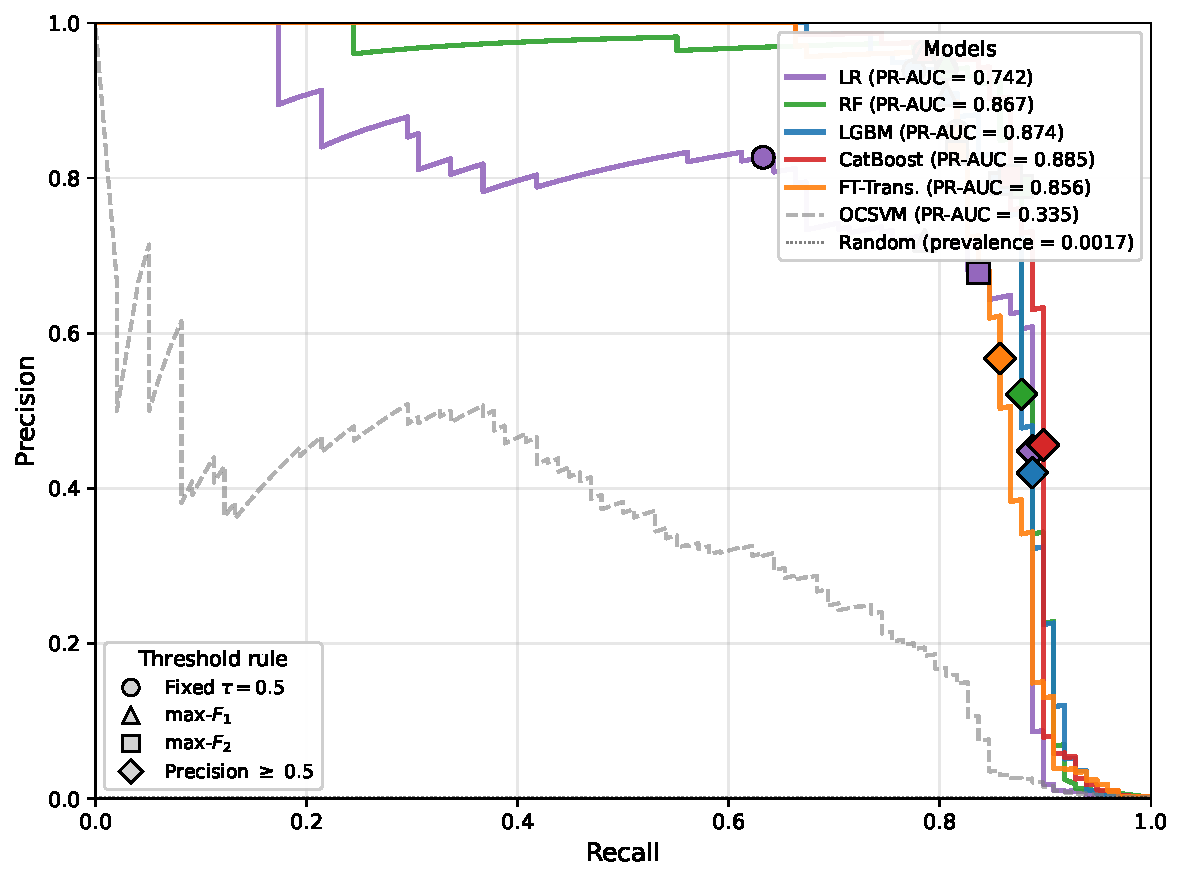
\includegraphics[width=0.48\textwidth]{figs/ulb_pr_curves_threshold.pdf}%
  \hfill
  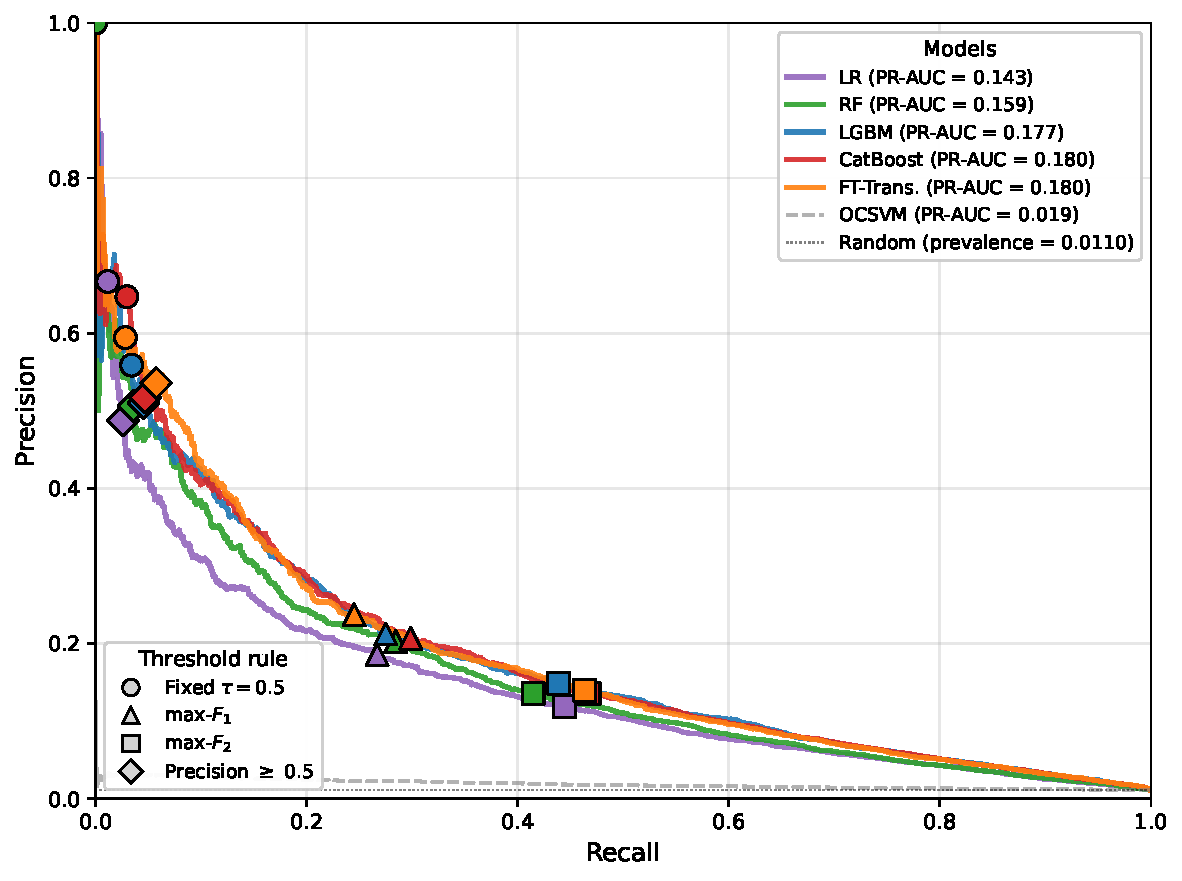
\includegraphics[width=0.48\textwidth]{figs/baf_pr_curves_threshold.pdf}
  \captionof{figure}{Precision--Recall curves for all models on ULB~2013 (left) and
    BAF~Base (right) under the baseline condition (strategy\,=\,None). Each curve
    represents the full operating space available to the model; the markers indicate
    where the four threshold rules studied in this paper land on that curve
    (\textbullet\ fixed~$\tau{=}0.5$; $\blacktriangle$~max-$F_1$;
    $\blacksquare$~max-$F_2$; $\blacklozenge$~Precision~$\geq$~0.5).
    OCSVM is shown as a dashed reference; threshold markers are omitted for OCSVM
    because its decision-function output is not on the probability scale.}
  \label{fig:prauc_baseline}
\end{minipage}\par\medskip

On ULB~2013, all supervised models achieve high PR-AUC ($>0.74$). CatBoost leads
at~0.885, followed by LGBM~(0.874), RF~(0.867), and the FT-Transformer~(0.856),
with Logistic Regression trailing substantially at~0.742 and OCSVM serving only as a
weak anomaly-detection baseline~(0.335). The performance gap between the non-linear
supervised models and LR reflects the capacity of tree-based and attention-based
classifiers to capture higher-order feature interactions even on PCA-anonymised inputs.
This pattern is consistent with the observation of \citet{shwartzziv2022tabular} that
tabular transformers are competitive with, but rarely superior to, gradient boosting
on small tabular datasets.

The geometry of the PR curves in the left panel of Fig.~\ref{fig:prauc_baseline} adds a
qualitative observation that the PR-AUC scalar alone cannot convey. Every supervised
curve maintains precision above~$\sim$0.8 across most of the recall range, so the four
threshold rules fall on visually overlapping operating points (the right portion of
each curve). The single exception is Logistic Regression, whose fixed-$\tau{=}0.5$
marker (purple circle) sits at recall~$\approx$0.63 --- well below the operating
cluster of the other models --- providing an immediate visual indication that, of all
supervised models on ULB, only LR leaves substantial recall unused under the default
threshold.

On BAF~Base, the picture changes substantially. All supervised models exhibit PR-AUC
near~$0.18$, reflecting the greater intrinsic difficulty of this large-scale dataset.
Notably, the FT-Transformer matches CatBoost exactly at PR-AUC~$=0.180$, suggesting
that attention-based architectures benefit from increased training data ($N\!=\!1$M
vs.\ $284$K) and close the gap with gradient boosting at this scale. LGBM~(0.177) and
RF~(0.159) complete the supervised tier, while OCSVM collapses~(0.019).

The right panel of Fig.~\ref{fig:prauc_baseline} previews the central finding of this
paper before the threshold-sensitivity tables formalise it. Under the BAF score
distribution, the four threshold rules no longer cluster on each model's curve as they
did on ULB; instead, they spread out to form a clear ladder. The fixed-$\tau{=}0.5$ rule
(circles) sits near zero recall in a high-precision regime, but at recall too low to
translate into useful $F_2$; max-$F_2$ (squares) lies at the rightmost portion of the
curve, trading precision for the recall the application actually needs; and max-$F_1$
(triangles) and Precision~$\geq$~0.5 (diamonds) occupy intermediate positions. The
geometric distance between the circle and the square along each curve is the visual
analogue of the order-of-magnitude $F_2$ swing that the next section quantifies.

\subsection{Threshold Sensitivity Analysis}
\label{subsec:threshold_results}

Tables~\ref{tab:threshold_ulb_f2}--\ref{tab:threshold_baf_alert} report $F_2$ and Alert
Rate under all four threshold strategies on both datasets.

\par\medskip\noindent\begin{minipage}{\linewidth}\centering
\captionof{table}{Threshold sensitivity on ULB~2013 --- $F_2$ by threshold strategy.}
\label{tab:threshold_ulb_f2}
\begin{tabular}{l c c c c}
\toprule
Model & Fixed ($0.5$) & max-$F_1$ & max-$F_2$ & Prec\,$\geq\!0.5$ \\
\midrule
LR         & 0.664 & 0.772 & 0.799 & 0.742 \\
RF         & 0.830 & 0.832 & 0.858 & 0.772 \\
LGBM       & 0.803 & 0.825 & 0.843 & 0.726 \\
CatBoost   & 0.816 & 0.816 & 0.853 & 0.752 \\
FT-Trans.  & 0.825 & 0.825 & 0.820 & 0.778 \\
OCSVM      & 0.420 & 0.498 & 0.527 & 0.455 \\
\bottomrule
\end{tabular}
\end{minipage}\par\medskip

\par\medskip\noindent\begin{minipage}{\linewidth}\centering
\captionof{table}{Threshold sensitivity on BAF~Base --- $F_2$ by threshold strategy.}
\label{tab:threshold_baf_f2}
\begin{tabular}{l c c c c}
\toprule
Model & Fixed ($0.5$) & max-$F_1$ & max-$F_2$ & Prec\,$\geq\!0.5$ \\
\midrule
LR         & 0.015 & 0.245 & 0.287 & 0.032 \\
RF         & 0.001 & 0.263 & 0.294 & 0.045 \\
LGBM       & 0.042 & 0.260 & 0.316 & 0.056 \\
CatBoost   & 0.037 & 0.274 & 0.314 & 0.058 \\
FT-Trans.  & 0.035 & 0.244 & 0.317 & 0.070 \\
OCSVM      & 0.031 & 0.071 & 0.081 & 0.000 \\
\bottomrule
\end{tabular}
\end{minipage}\par\medskip

\par\medskip\noindent\begin{minipage}{\linewidth}\centering
\captionof{table}{Threshold sensitivity on BAF~Base --- Alert Rate (\%) by threshold strategy.}
\label{tab:threshold_baf_alert}
\begin{tabular}{l c c c c}
\toprule
Model & Fixed ($0.5$) & max-$F_1$ & max-$F_2$ & Prec\,$\geq\!0.5$ \\
\midrule
LR         & 0.02 & 1.59 & 4.14 & 0.06 \\
RF         & 0.00 & 1.55 & 3.36 & 0.08 \\
LGBM       & 0.07 & 1.43 & 3.25 & 0.10 \\
CatBoost   & 0.05 & 1.59 & 3.80 & 0.10 \\
FT-Trans.  & 0.05 & 1.14 & 3.66 & 0.12 \\
OCSVM      & 1.03 & 4.06 & 7.32 & 0.00 \\
\bottomrule
\end{tabular}
\end{minipage}\par\medskip

On ULB~2013, threshold choice has a moderate but measurable impact. For CatBoost and
LGBM, the fixed~$\tau=0.5$ already performs well ($F_2\!\approx\!0.81$), because the
predicted scores are sufficiently separated that the default operating point falls in
a region where both classes are well discriminated. Logistic Regression benefits most
from threshold optimisation: $F_2$ improves from~$0.664$ under the default to~$0.799$
under max-$F_2$, a~$20\%$ relative gain. Crucially, model rankings are preserved across
all four strategies on ULB.

On BAF~Base, the magnitude of the effect changes by an order of magnitude. The
fixed~$\tau=0.5$ severely degrades detection performance: $F_2$ falls below~$0.04$ for
every supervised model, and RF in particular produces essentially no positive
predictions ($F_2\!=\!0.001$, Alert Rate\,=\,$0.00\%$). The underlying reason is that
fraud scores on BAF are concentrated in the~$0.04$--$0.10$ range, so the~$0.5$ default
discards almost every positive prediction. Switching to max-$F_2$ recovers substantial
performance: CatBoost's $F_2$ improves from~$0.037$ to~$0.314$, a ${\approx}8.5\times$
gain, and the FT-Transformer improves from~$0.035$ to~$0.317$, a~$9\times$ gain.

The Alert Rate table (Table~\ref{tab:threshold_baf_alert}) makes the workload
implications visible. The max-$F_2$ strategy requires investigators to review~$3.2$--$4.1\%$
of all transactions (${\approx}32\,000$--$41\,000$ per million), whereas the
Precision~$\geq\!0.5$ strategy reduces this load to~$0.06$--$0.12\%$ at the cost of
substantially lower recall. The empirical regularity is therefore not merely that
threshold choice affects performance, but that on BAF it changes the operational
classification of the system from one that flags almost nothing to one that detects
$41$--$47\%$ of fraud --- a qualitative change in operating regime that no model-level
or strategy-level intervention reproduces.

\subsection{Full Factorial Analysis: Imbalance Strategy \texorpdfstring{$\times$}{x} Model}
\label{subsec:factorial}

Tables~\ref{tab:factorial_ulb_prauc}--\ref{tab:factorial_baf_f2} present PR-AUC and
$F_2$ under all strategy--model combinations, and Figure~\ref{fig:heatmaps} shows the
corresponding $\Delta$PR-AUC heatmaps (strategy minus None baseline).

\par\medskip\noindent\begin{minipage}{\linewidth}\centering
\captionof{table}{PR-AUC by model $\times$ strategy on ULB~2013. Bold: best result per row.}
\label{tab:factorial_ulb_prauc}
\begin{tabular}{l c c c c c c c}
\toprule
Model & None & RUS & ROS & SMOTE & SM+T & SMOTEENN & Weights \\
\midrule
LR         & \textbf{0.742} & 0.674 & 0.711 & 0.721 & 0.721 & 0.732 & 0.709 \\
RF         & 0.867 & 0.669 & \textbf{0.873} & 0.870 & 0.870 & 0.853 & 0.859 \\
LGBM       & \textbf{0.874} & 0.678 & 0.727 & 0.724 & 0.724 & 0.724 & 0.726 \\
CatBoost   & \textbf{0.885} & 0.617 & 0.879 & 0.857 & 0.857 & 0.846 & 0.875 \\
FT-Trans.  & \textbf{0.856} & 0.650 & 0.836 & 0.845 & 0.845 & 0.772 & 0.783 \\
\bottomrule
\end{tabular}
\end{minipage}\par\medskip

\par\medskip\noindent\begin{minipage}{\linewidth}\centering
\captionof{table}{PR-AUC by model $\times$ strategy on BAF~Base. Bold: best result per row.}
\label{tab:factorial_baf_prauc}
\begin{tabular}{l c c c c c c c}
\toprule
Model & None & RUS & ROS & SMOTE & SM+T & SMOTEENN & Weights \\
\midrule
LR         & \textbf{0.143} & 0.137 & 0.137 & 0.135 & 0.135 & 0.136 & 0.122 \\
RF         & \textbf{0.159} & 0.135 & 0.149 & 0.120 & 0.120 & 0.124 & 0.146 \\
LGBM       & 0.177 & 0.171 & \textbf{0.181} & 0.146 & 0.146 & 0.158 & 0.181 \\
CatBoost   & 0.180 & 0.178 & \textbf{0.185} & 0.154 & 0.154 & 0.165 & 0.184 \\
FT-Trans.  & \textbf{0.180} & 0.159 & 0.166 & 0.106 & 0.106 & 0.124 & 0.175 \\
\bottomrule
\end{tabular}
\end{minipage}\par\medskip

\par\medskip\noindent\begin{minipage}{\linewidth}\centering
\captionof{table}{$F_2$ by model $\times$ strategy on BAF~Base (max-$F_2$ threshold). Bold: best result per row.}
\label{tab:factorial_baf_f2}
\begin{tabular}{l c c c c c c c}
\toprule
Model & None & RUS & ROS & SMOTE & SM+T & SMOTEENN & Weights \\
\midrule
LR         & \textbf{0.287} & 0.283 & 0.283 & 0.280 & 0.280 & 0.282 & 0.267 \\
RF         & 0.294 & 0.288 & \textbf{0.303} & 0.280 & 0.280 & 0.280 & 0.296 \\
LGBM       & 0.316 & 0.318 & 0.319 & 0.293 & 0.293 & 0.300 & \textbf{0.320} \\
CatBoost   & 0.314 & \textbf{0.317} & 0.316 & 0.303 & 0.303 & 0.309 & 0.317 \\
FT-Trans.  & \textbf{0.316} & 0.289 & 0.310 & 0.255 & 0.255 & 0.269 & 0.301 \\
\bottomrule
\end{tabular}
\end{minipage}\par\medskip

\par\medskip\noindent\begin{minipage}{\linewidth}\centering
  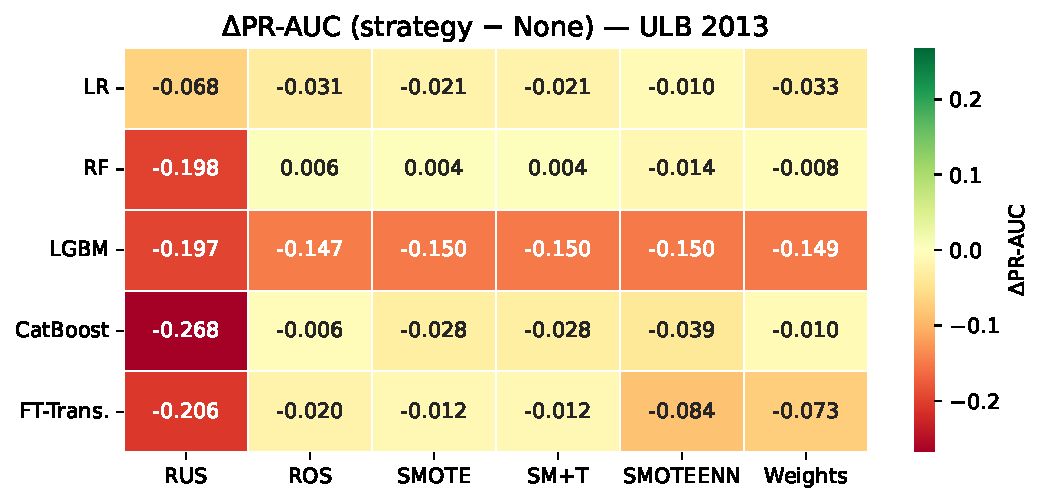
\includegraphics[width=0.48\textwidth]{figs/ulb_heatmap_prauc.pdf}%
  \hfill
  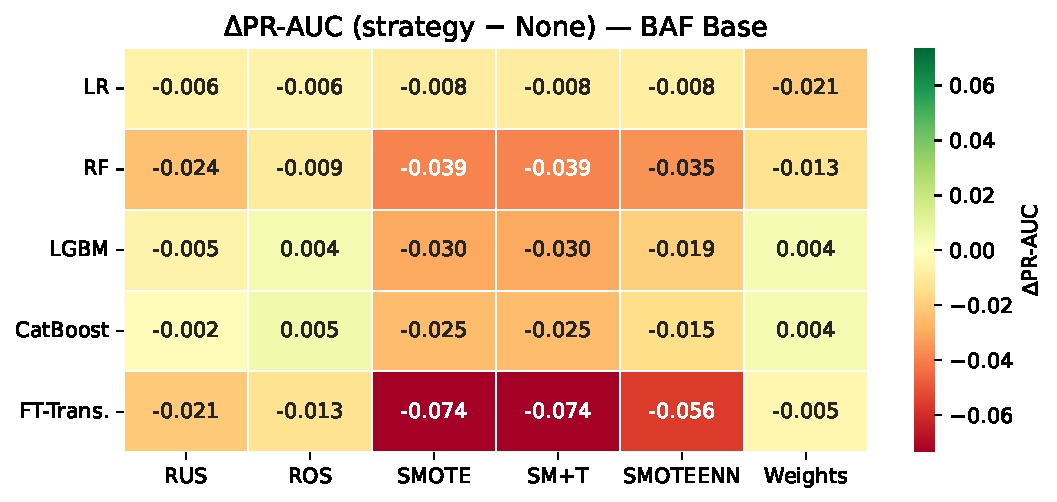
\includegraphics[width=0.48\textwidth]{figs/baf_heatmap_prauc.pdf}
  \captionof{figure}{$\Delta$PR-AUC (strategy minus None baseline) heatmaps on ULB~2013 (left)
    and BAF~Base (right). Green cells indicate improvement; red cells indicate degradation.}
  \label{fig:heatmaps}
\end{minipage}\par\medskip

On ULB~2013, the unmodified baseline is optimal for LGBM, CatBoost, and the
FT-Transformer. Random Forest is the only model that benefits from oversampling, with
ROS raising PR-AUC from~$0.867$ to~$0.873$. ROS substantially degrades LGBM
($0.874\!\to\!0.727$, $-17\%$), a pattern consistent with random duplication of
minority samples disrupting its gradient landscape. A noteworthy observation is that
SMOTE and SMOTE+Tomek produce identical PR-AUC values across all models on both
datasets; the practical implication is that the additional preprocessing cost of
SMOTE+Tomek delivers no empirical benefit on fraud data of this prevalence
(the mechanism is examined in Section~\ref{subsec:disc_strategy}).

On BAF~Base, the well-tuned gradient-boosted models handle imbalance natively: no
strategy improves the PR-AUC of LGBM or CatBoost beyond the baseline by more than~$0.005$.
SMOTE, however, degrades the FT-Transformer by~$41\%$ on BAF~Base ($0.180\!\to\!0.106$),
compared to only~$14\%$ for CatBoost ($0.180\!\to\!0.154$). The same asymmetry appears
in $F_2$ and is exactly reproduced by SMOTE+Tomek; the underlying mechanism is
discussed in Section~\ref{subsec:disc_architecture}.

\subsection{Confidence Intervals and Computational Cost}
\label{subsec:ci_cost}

Tables~\ref{tab:ci_baf} and~\ref{tab:cost_baf} report bootstrap confidence intervals
and training cost on BAF Base.

\par\medskip\noindent\begin{minipage}{\linewidth}\centering
\captionof{table}{95\% Bootstrap CI for PR-AUC and ROC-AUC on BAF Base (strategy\,=\,None, $B\!=\!1\,000$).}
\label{tab:ci_baf}
\begin{tabular}{l c c c c}
\toprule
Model & PR-AUC & 95\% CI & ROC-AUC & 95\% CI \\
\midrule
LR         & 0.143 & [0.131, 0.158] & 0.875 & [0.867, 0.882] \\
RF         & 0.159 & [0.145, 0.175] & 0.878 & [0.870, 0.885] \\
LGBM       & 0.177 & [0.162, 0.194] & 0.898 & [0.892, 0.905] \\
CatBoost   & 0.180 & [0.164, 0.197] & 0.898 & [0.892, 0.904] \\
FT-Trans.  & 0.180 & [0.164, 0.197] & 0.897 & [0.891, 0.904] \\
OCSVM      & 0.019 & [0.018, 0.021] & 0.628 & [0.616, 0.639] \\
\bottomrule
\end{tabular}
\end{minipage}\par\medskip

\par\medskip\noindent\begin{minipage}{\linewidth}\centering
\captionof{table}{Computational cost on BAF Base (strategy\,=\,None). Tuning includes 50 Optuna trials.}
\label{tab:cost_baf}
\begin{tabular}{l r r r}
\toprule
Model & Tuning (s) & Training (s) & Inference (s) \\
\midrule
LR         & 55,070 & 83.9 & 0.321 \\
RF         & 105,313 & 1,494.0 & 21.075 \\
LGBM       & 1,243 & 16.1 & 1.387 \\
CatBoost   & 7,010 & 36.7 & 0.249 \\
FT-Trans.  & 46,550 & 346.9 & 2.419 \\
OCSVM      & --- & 919.6 & 71.579 \\
\bottomrule
\end{tabular}
\end{minipage}\par\medskip

The bootstrap CIs in Table~\ref{tab:ci_baf} indicate that the FT-Transformer and
CatBoost confidence intervals overlap exactly on BAF (both [0.164, 0.197]),
providing no statistical basis for preferring one over the other at the current
sample size. The width of these intervals reflects the intrinsic difficulty of
estimating PR-AUC under extreme imbalance: even with $N\!=\!1$M, the bootstrap
distribution carries substantial variance because the relevant region of the
precision-recall curve is determined by approximately~$11\,000$ fraud cases.

Table~\ref{tab:cost_baf} brings out a sharp computational asymmetry. LGBM achieves a
PR-AUC of~$0.177$ with only~$16$~seconds of training time, while the FT-Transformer
requires~$347$~seconds of GPU-accelerated training for a statistically equivalent
result of~$0.180$. Optuna tuning shows an even larger gap: LightGBM's search completes
in~$1\,243$~s, against~$46\,550$~s for the FT-Transformer, primarily because LGBM's
tree-based training is CPU-parallelisable and avoids epoch-based overhead.

%% ════════════════════════════════════════════════════════════════════════════
\section{Discussion}
\label{sec:discussion}
%% ════════════════════════════════════════════════════════════════════════════

\subsection{Score Geometry under Extreme Imbalance}
\label{subsec:disc_threshold}

The asymmetry between the two datasets is best understood by looking at where the
predicted score distributions place the operating point implied by each threshold rule.
On ULB~2013, the spread of PR-AUC across models is large
($0.742$--$0.885$), while the spread of $F_2$ across threshold strategies is much
smaller; on BAF~Base, this ranking reverses, with the PR-AUC range collapsing into a
$0.04$-point band ($0.143$--$0.180$) while the $F_2$ range across threshold strategies
spans nearly the full unit interval ($0.001$--$0.317$). What changes between the two
benchmarks is not the relative quality of the classifiers but the geometry of the score
space in which they operate.

On ULB, supervised models assign fraud transactions probability scores that are
substantially separated from the legitimate-class mass; the operating point implied by
$\tau=0.5$ therefore lies in a region where both densities are well discriminated, and
threshold tuning yields only second-order gains. On BAF, the higher prevalence is
deceptive: the per-feature discriminative signal is weaker, and predicted scores
collapse into the~$0.04$--$0.10$ band irrespective of model. The default $\tau=0.5$ then
sits in the right tail of a heavily compressed distribution where almost no probability
mass exists, leaving the system in a regime in which positive predictions are rare and
$F_2$ approaches zero. The fixed default is therefore not catastrophic in any model-
or strategy-specific sense; it is operationally unsuitable for any classifier whose
score distribution is compressed in this way, which under extreme imbalance is the
typical case rather than the exception.

This geometric reading also clarifies what changes when the threshold is moved. Sliding
$\tau$ leftwards from~$0.5$ into the bulk of the compressed score distribution is the
mechanism by which max-$F_2$ recovers the missing recall: the relevant region of the PR
curve is the steep portion close to the prevalence baseline, and the validation-optimal
threshold is precisely the operating point that enters that region. The same exercise
on ULB only shifts an already well-placed operating point along a shallow plateau of
the PR curve, which is why threshold sensitivity there is real but limited. The
relevant practical statement is therefore not that ``threshold tuning matters'' in the
abstract, but that score compression under extreme imbalance produces operating-point
instability whose only deployable remedy is explicit, validation-calibrated threshold
selection.

The Alert Rate table (Table~\ref{tab:threshold_baf_alert}) makes the trade-off
operational. The max-$F_2$ strategy maximises recall at a precision cost that requires
investigators to review~$3.2$--$4.1\%$ of all transactions, whereas Precision~$\geq\!0.5$
reduces the workload to~$0.06$--$0.12\%$ in exchange for substantially lower recall.
Which strategy is appropriate is therefore deployment-context dependent: a high-volume
automated system can absorb higher alert rates, whereas a human-investigator team with
bounded capacity will favour a precision-constrained strategy. In both cases the
threshold must be selected explicitly, in awareness of the metric trade-offs, rather
than inherited unexamined from the software default.

\subsection{Why No Imbalance Strategy Dominates}
\label{subsec:disc_strategy}

The factorial results confirm that no single imbalance handling strategy improves
performance across all model families and both datasets, and the underlying reasons
can be read off the score-geometry argument of the previous subsection.

The empirical equivalence between SMOTE and SMOTE+Tomek admits a straightforward
mechanistic explanation. Tomek Links cleaning removes majority-class examples that lie
on the decision boundary near synthetic minorities; when the minority class is as rare
as~$0.17\%$--$1.1\%$, the synthetic SMOTE examples are too sparse relative to the
majority population for any Tomek-linked pair to be identified. The cleaned set therefore
coincides exactly with the SMOTE output. The implication for practice is that adopting
SMOTE+Tomek over plain SMOTE imposes additional preprocessing cost without altering the
training distribution on data of this sparsity.

Class~Weights is, on balance, the safest default across model families. On BAF it
neither degrades nor materially improves GBDT or FT-Transformer performance
(LGBM~$+0.004$, CatBoost~$+0.004$). The principal exception is LGBM on ULB, where
Class~Weights drops PR-AUC from~$0.874$ to~$0.726$ ($-17\%$); however, every other
strategy degrades LGBM on ULB by a comparable margin (ROS: $-17\%$; SMOTE: $-17\%$),
which indicates that LGBM on ULB is sensitive to any deviation from the unmodified
baseline rather than to Class~Weights specifically. In the absence of dataset-specific
prior evidence, Class~Weights is therefore the recommended starting point because it
modifies the loss surface rather than the empirical distribution of the training data
and consequently introduces fewer second-order distortions.

The remaining factorial pattern is consistent with the broader picture: on ULB only
Random Forest benefits from oversampling (ROS~$+0.6\%$ PR-AUC), and on BAF no strategy
improves LGBM or CatBoost by more than~$0.005$ PR-AUC. Modern gradient boosting
implementations handle moderate imbalance natively via internal tree-level reweighting,
and the marginal gains from external resampling are therefore swamped by the second-order
distortions resampling itself introduces.

\subsection{Architecture-Specific Imbalance Sensitivity}
\label{subsec:disc_architecture}

The contrast between FT-Transformer and CatBoost under SMOTE is the clearest
architecture-level signal in the factorial. On BAF~Base, SMOTE degrades the
FT-Transformer's PR-AUC by~$41\%$ ($0.180\!\to\!0.106$), against only~$14\%$ for
CatBoost ($0.180\!\to\!0.154$). The asymmetry is mirrored in $F_2$ and reproduced
exactly by SMOTE+Tomek.

The most plausible mechanistic account is that synthetic minority examples generated by
SMOTE perturb the joint feature distribution that the attention mechanism implicitly
estimates. Gradient-based optimisation of attention weights is sensitive to the global
density of the training distribution, because the softmax over tokens couples updates
across the entire input space; tree-based learners, by contrast, take split decisions on
local statistics and are largely indifferent to global density shifts that do not move
the chosen split points. Synthetic interpolation in feature space is therefore a more
disruptive intervention for a transformer than for a tree ensemble. A full mechanistic
account, including FT-Transformer attention diagnostics and cross-domain robustness
analysis, is provided in a companion paper currently in preparation.

The deployment implication is unambiguous: practitioners applying SMOTE to a neural
tabular model should validate against a Class~Weights baseline before adopting the
strategy, since the expected gain observed for tree-based learners does not carry over
to attention-based architectures.

\subsection{Decision Framework}
\label{subsec:disc_framework}

Table~\ref{tab:decision_framework} synthesises the experimental evidence into a
decision framework for fraud detection practitioners. Each row maps a deployment
scenario to the recommended model, imbalance strategy, and threshold strategy, derived
from the results in Section~\ref{sec:results}.

\par\medskip\noindent\begin{minipage}{\linewidth}\centering
\captionof{table}{Decision framework: recommended configuration by deployment scenario.
  Recommendations are derived from the results in Section~\ref{sec:results}.}
\label{tab:decision_framework}
\begin{tabular}{p{3.8cm} l l l}
\toprule
Deployment scenario & Model & Strategy & Threshold \\
\midrule
High recall, small dataset   & CatBoost  & None / ROS     & max-$F_2$      \\
Balanced $F_1$, small dataset & CatBoost  & None          & max-$F_1$      \\
High recall, large dataset   & LGBM      & None / Weights & max-$F_2$      \\
Balanced $F_1$, large dataset & CatBoost  & ROS           & max-$F_1$      \\
Low investigation budget     & CatBoost  & None           & Prec\,$\geq\!0.5$ \\
Tree-based + low compute     & LGBM      & None           & max-$F_2$      \\
Tabular transformer (DL)     & FT-Trans. & Class Weights  & max-$F_2$      \\
\bottomrule
\end{tabular}
\end{minipage}\par\medskip

Several patterns emerge from the framework. CatBoost is the default choice for
in-domain deployment, given its consistently top-tier performance across both datasets.
When investigation capacity is limited, the Precision~$\geq\!0.5$ rule is recommended:
it guarantees at least one genuine fraud per two alerts, keeping investigator workload
manageable at the cost of lower recall. When the deployment constraint is a tree-based
architecture with a minimal compute footprint --- a common requirement for systems
compatible with tree-path SHAP explainers and constrained tuning budgets --- LGBM is
the natural choice: both LGBM and CatBoost expose tree-path SHAP through the standard
\texttt{TreeExplainer} interface, but LGBM reaches statistically equivalent PR-AUC at
considerably lower computational cost (tuning is $5.6\times$ faster and training
$2.3\times$ faster than CatBoost on BAF Base, see Table~\ref{tab:cost_baf}). For
FT-Transformer deployments, Class~Weights is preferred to SMOTE-based interventions for
the architecture-specific reasons developed in
Section~\ref{subsec:disc_architecture}.

A more concise way to summarise the framework is that, for any deployment on data
resembling the BAF regime (large-scale, moderate imbalance, score compression), the
first design decision should not be model choice but explicit threshold selection on
a held-out validation set under a recall-weighted criterion. The empirical justification
is that on BAF the range of PR-AUC across all supervised models spans only~$0.04$
points, whereas the range of $F_2$ across threshold strategies spans~$0.31$ points.

%% ════════════════════════════════════════════════════════════════════════════
\section{Conclusion}
\label{sec:conclusion}
%% ════════════════════════════════════════════════════════════════════════════

The central message of this work is that, under extreme class imbalance, the behaviour
of a fraud detection system is shaped less by the choice of classifier than by the
geometry of the predicted score distribution and the rule that converts those scores
into operational decisions. Treating the decision threshold as a first-class
experimental variable, calibrated exclusively on inner validation folds, exposes an
order-of-magnitude effect that no factorial combination of model and resampling
strategy reproduces. Once this score-geometry view is adopted, the recurrent
methodological failures of the fraud detection literature --- resampling leakage,
test-set threshold selection, and reliance on ROC-AUC --- appear as different facets
of a single underlying issue, namely the failure to characterise model behaviour at
the operating point that the deployment actually uses.

Beyond fraud detection specifically, this perspective has implications for any
classification setting characterised by score compression under low prevalence.
Reported performance gains attributable to model choice, architecture, or imbalance
strategy may be small relative to the gains obtainable through explicit threshold
selection on a held-out validation set, and benchmarking protocols that conflate the
two will systematically misrepresent which design decisions are first-order. The
decision framework in Table~\ref{tab:decision_framework} operationalises this view
into actionable guidance for practitioners.

Two limitations bound the scope of these conclusions. The Optuna budget of 50 trials
may under-explore the FT-Transformer's search space relative to the classical models,
whose smaller spaces are more efficiently covered under TPE sampling. In addition, the
BAF dataset is synthetically generated, and although it is calibrated to resemble
real bank account application fraud, production systems may exhibit additional
complexities --- label noise, adversarial adaptation, temporal feedback loops --- that
are not captured here.

Several extensions of the present work follow naturally. The four threshold rules
studied here are static criteria calibrated once on a held-out validation set, whereas
production fraud streams exhibit concept drift; an open question is whether periodic
recalibration of $\tau$ alone is sufficient to maintain operational $F_2$ over time,
or whether full model retraining is required. Threshold rules that explicitly enforce
an investigation-team capacity constraint --- for instance a fixed alert budget per
period --- would also map more directly onto the operational decisions made by
fraud-detection teams. Finally, asymmetric loss functions designed natively for
extreme imbalance, such as focal loss or direct $F_\beta$ optimisation, would provide
a principled alternative to both data-level resampling and uniform class reweighting,
and are particularly attractive for architectures such as the FT-Transformer where
data-level interventions degrade performance substantially.

A mechanistic explanation of \emph{why} gradient-boosted models match or outperform
tabular transformers on fraud data --- including FT-Transformer attention diagnostics
and cross-domain robustness analysis across the five BAF variants --- is provided in
a companion paper.

\printcredits

\bibliographystyle{cas-model2-names}
\bibliography{cas-refs}

\end{document}
